\documentclass[11pt,oneside]{article}

\usepackage[T1]{fontenc}
\usepackage[utf8]{inputenc}
\usepackage{lmodern}
\usepackage[margin=0.82in]{geometry}
\usepackage{amsmath,amssymb,amsthm,mathtools}
\usepackage{booktabs,tabularx,array}
\usepackage{graphicx}
\usepackage{xcolor}
\usepackage{microtype}
\usepackage{enumitem}
\usepackage{hyperref}
\usepackage{fancyhdr}
\usepackage[most]{tcolorbox}

\definecolor{navy}{HTML}{12355B}
\definecolor{blue}{HTML}{1675A9}
\definecolor{pale}{HTML}{EEF5FA}
\definecolor{warning}{HTML}{9B3A22}
\hypersetup{colorlinks=true,linkcolor=navy,urlcolor=blue,citecolor=blue}
\pagestyle{fancy}
\fancyhf{}
\lhead{\textsc{Financial Engineering Lab}}
\rhead{\textsc{SPX Volatility Surface}}
\cfoot{\thepage}
\setlength{\headheight}{14pt}
\setlist[itemize]{leftmargin=1.3em,itemsep=2pt}

\newtheorem{proposition}{Proposition}
\newtheorem{assumption}{Assumption}
\newtcolorbox{claimbox}[1][]{colback=pale,colframe=navy,title=#1,fonttitle=\bfseries}
\newtcolorbox{riskbox}[1][]{colback=red!3,colframe=warning,title=#1,fonttitle=\bfseries}
\newcommand{\E}{\mathbb{E}}
\newcommand{\Q}{\mathbb{Q}}
\newcommand{\R}{\mathbb{R}}
\newcommand{\dd}{\,\mathrm{d}}

\title{\vspace{-1.2cm}\textbf{\Huge An Arbitrage-Aware SPX Volatility Surface}\\[0.4em]
       \Large Identification, Constrained SVI, Heston Calibration, and Honest Validation}
\author{Financial Engineering Lab}
\date{Reference session: 27 August 2026}

\begin{document}
\maketitle

\begin{abstract}
This study constructs an auditable volatility surface from a delayed public SPX
option-chain snapshot. Forward prices and discount factors are identified by robust
put--call parity, implied volatilities are obtained by no-arbitrage inversion, and
each maturity is fitted with a constrained raw-SVI smile. A five-parameter Heston
model is then estimated by multi-start nonlinear least squares on a deterministic
training set and judged on strikes excluded before calibration. The held-out
IV-equivalent root-mean-square error is 0.01464, versus 0.04459 for a maturity-level
flat-volatility null. This improvement is economically substantial but not a
certificate of truth: quotes are asynchronous delayed transactions, one parity fit
touches its economically imposed discount bound, and the unconstrained best Heston
fit violates the Feller sufficient condition. Those weaknesses are reported as
results rather than hidden as implementation details.
\end{abstract}

\begin{claimbox}[What this paper can defend]
The repository can reproduce every table and figure from an immutable raw snapshot;
the surface satisfies explicit dense-grid static-arbitrage diagnostics; the Heston
comparison uses data not seen during fitting; and numerical uncertainty, multi-start
stability, data limitations, and failed structural restrictions are visible.
\end{claimbox}

\section{Research question and falsification design}

The question is narrow: \emph{does a single stochastic-volatility parameter vector
explain the cross-section of SPX smiles better than a transparent flat-volatility
benchmark, without allowing the preliminary surface fit to manufacture static
arbitrage?} The following statements were fixed in code before calibration.

\begin{enumerate}
  \item The observable information set ends at the common reference session.
  \item Four expirations are selected near 30, 90, 180, and 365 calendar days, with
        standard monthly contracts included in the candidate pool.
  \item Every fourth strike within each selected calibration slice is held out
        deterministically. Heston parameters never see those observations.
  \item The null assigns each maturity the liquidity-weighted training-sample mean
        implied volatility.
  \item Failure is possible: negative butterfly density, calendar inversion,
        unstable optimization, implausible parity, or no held-out improvement would
        all weaken the model.
\end{enumerate}

The design is a cross-sectional specification test, not a forecast. The option
prices are risk-neutral objects and do not estimate physical return probabilities.

\section{Contracts, observations, and information time}

SPX options are used because their European exercise convention makes the
put--call-parity equality coherent. The underlying and chains came from a delayed
public Yahoo Finance interface through \texttt{yfinance}. It is a convenient
research feed, not an exchange-certified historical record. The raw response,
ingestion timestamp, library version, candidate-expiration audit, and SHA-256
manifest are committed with the analysis.

Displayed bid and ask fields were too sparse to define a usable common cross-section.
The study therefore uses the latest reported transaction for each contract whose
timestamp falls within the reference session (with a short post-close reporting
allowance). Call and put transactions at a common strike are generally asynchronous.
Liquidity weights and the call--put timestamp gap enter the parity fit, but this
cannot eliminate staleness.

\begin{assumption}[Measurement equation]
For contract $i$, the observed transaction price satisfies
\[
  P_i^{\mathrm{obs}}=P_i^{\ast}+\varepsilon_i,
\]
where $P_i^\ast$ is a synchronous frictionless value and $\varepsilon_i$ includes
bid--ask location, reporting delay, discreteness, and stale-price error. The
pipeline propagates a parity-residual scale as an empirical noise benchmark; it
does not interpret that scale as an independent Gaussian standard error.
\end{assumption}

\section{Forward and discount identification}

For European calls and puts with common strike $K$ and maturity $T$,
\begin{equation}
  C(K,T)-P(K,T)=D(T)\,[F(T)-K]=\alpha_T-\beta_TK,
  \qquad \alpha_T=D(T)F(T),\quad\beta_T=D(T).
  \label{eq:parity}
\end{equation}
Thus a cross-section of paired strikes identifies the slope $-D(T)$ and intercept
$D(T)F(T)$. Estimation uses a soft-$L^1$ loss and liquidity weights. To prevent an
asynchronous public chain from implying economically nonsensical discounting,
$D(T)$ is bounded by continuously compounded rates between zero and 15 percent.

\begin{proposition}[Parity recovery]
If equation \eqref{eq:parity} holds at two distinct strikes and $D(T)>0$, then
$D(T)$ and $F(T)$ are uniquely identified.
\end{proposition}
\begin{proof}
Subtract parity at $K_1$ and $K_2$. Since $K_1\ne K_2$,
\[
 D(T)=-\frac{[C_1-P_1]-[C_2-P_2]}{K_1-K_2}.
\]
Substitution into either equation gives
$F(T)=K_i+[C_i-P_i]/D(T)$. Uniqueness follows from the nonzero strike difference.
\end{proof}

\begin{table}[ht]
\centering
\caption{Robust put--call-parity estimates. Prices and strikes are index points.}
\resizebox{\textwidth}{!}{\begin{tabular}{lrrrrrr}
\toprule
expiration & maturity\_years & forward & discount & parity\_rmse & parity\_pairs & discount\_at\_upper\_bound \\
\midrule
2026-09-18 & 0.0602 & 7740.8471 & 0.9978 & 4.9360 & 7 & False \\
2026-11-20 & 0.2327 & 7784.2754 & 1.0000 & 11.1077 & 7 & True \\
2027-02-19 & 0.4819 & 7872.5407 & 0.9667 & 1.9225 & 5 & False \\
2027-08-20 & 0.9802 & 8011.1433 & 0.9486 & 6.0432 & 10 & False \\
\bottomrule
\end{tabular}
}
\end{table}

\begin{riskbox}[Identification warning]
The November discount estimate touches its upper bound $D=1$. The fitted forward is
usable as a regularized nuisance estimate, but the corresponding zero rate is not
treated as an economic discovery. This boundary event is preserved in the
diagnostics and provenance.
\end{riskbox}

\section{Black inversion and total variance}

With forward $F$, discount $D$, volatility $\sigma$, and
$d_{1,2}=[\log(F/K)\pm\tfrac12\sigma^2T]/(\sigma\sqrt{T})$, Black's forward formula is
\[
 C=D[F\Phi(d_1)-K\Phi(d_2)],\qquad
 P=D[K\Phi(-d_2)-F\Phi(-d_1)].
\]
Only out-of-the-money options are retained: puts for $K<F$ and calls for $K\ge F$.
The implied volatility is the unique root when the observed price lies strictly
inside the no-arbitrage bounds. Root finding uses a bracketed Brent solver, avoiding
the vega instability of an unconstrained Newton step.

Log-forward moneyness and total implied variance are
\[
  k=\log(K/F),\qquad w(k,T)=\sigma_{\mathrm{imp}}(k,T)^2T.
\]
Total variance, rather than volatility, is the natural object for both SVI fitting
and calendar-spread diagnostics.

\section{Constrained SVI surface}

Each maturity uses the raw-SVI parameterization
\begin{equation}
 w(k)=a+b\left[\rho(k-m)+\sqrt{(k-m)^2+\sigma^2}\right],
 \label{eq:svi}
\end{equation}
with $b\ge0$, $|\rho|<1$, $\sigma>0$, and
$a+b\sigma\sqrt{1-\rho^2}\ge0$. The fit minimizes a liquidity-weighted squared
error in total variance. Numerical constraints are checked on a grid wider than the
observed strikes, not only at quoted points.

For a twice differentiable total-variance smile, the normalized state-price-density
factor is
\begin{equation}
g(k)=
\left(1-\frac{k w'(k)}{2w(k)}\right)^2
-\frac{[w'(k)]^2}{4}\left(\frac{1}{w(k)}+\frac14\right)
+\frac12w''(k).
\label{eq:g}
\end{equation}
A nonnegative $g$ is the relevant butterfly-arbitrage diagnostic under the standard
SVI transformation. The implementation also enforces finite Lee-wing slopes and
tests $w(k,T_{j+1})-w(k,T_j)\ge0$ on a common grid. If needed, the later slice receives
the smallest vertical total-variance shift that repairs the grid; no such shift was
needed in this snapshot.

\begin{table}[ht]
\centering
\caption{SVI errors and dense-grid arbitrage diagnostics.}
\resizebox{\textwidth}{!}{\begin{tabular}{lrrrrrrrrr}
\toprule
expiration & quotes & iv\_rmse & iv\_mae & inside\_empirical\_noise\_fraction & minimum\_total\_variance & minimum\_butterfly\_g & minimum\_calendar\_variance\_gap & left\_wing\_slope & right\_wing\_slope \\
\midrule
2026-09-18 & 152 & 0.00446 & 0.00363 & 0.90789 & 0.00062 & 0.00000 & NaN & 0.05433 & 0.05015 \\
2026-11-20 & 115 & 0.00215 & 0.00157 & 0.98261 & 0.00314 & 0.05997 & 0.00026 & 0.09928 & 0.05787 \\
2027-02-19 & 64 & 0.00147 & 0.00109 & 0.75000 & 0.00725 & 0.16569 & 0.00059 & 0.12893 & 0.05159 \\
2027-08-20 & 60 & 0.00126 & 0.00097 & 0.80000 & 0.01738 & 0.31977 & 0.00572 & 0.16300 & 0.05163 \\
\bottomrule
\end{tabular}
}
\end{table}

\begin{figure}[p]
\centering
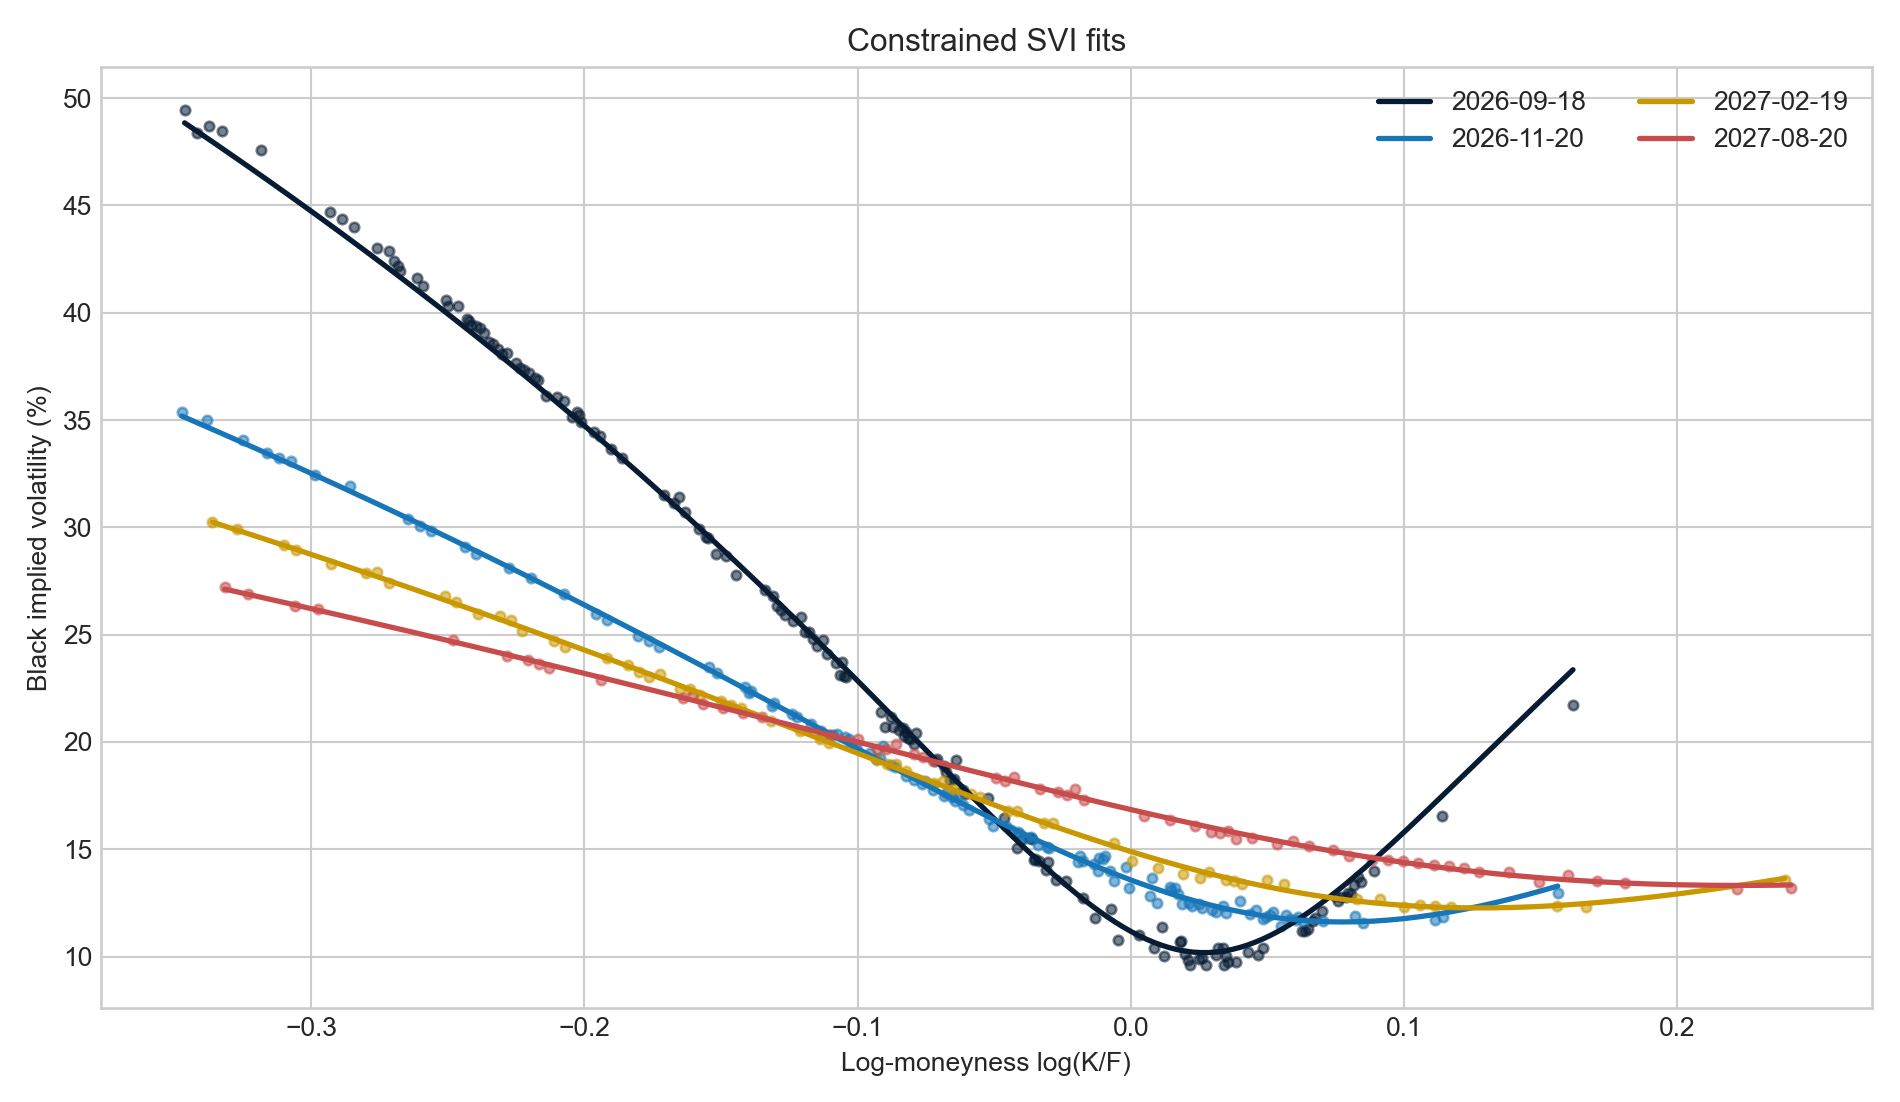
\includegraphics[width=.96\textwidth]{output/svi_fitted_smiles.png}
\caption{Observed implied volatilities and constrained SVI fits.}
\vspace{1em}
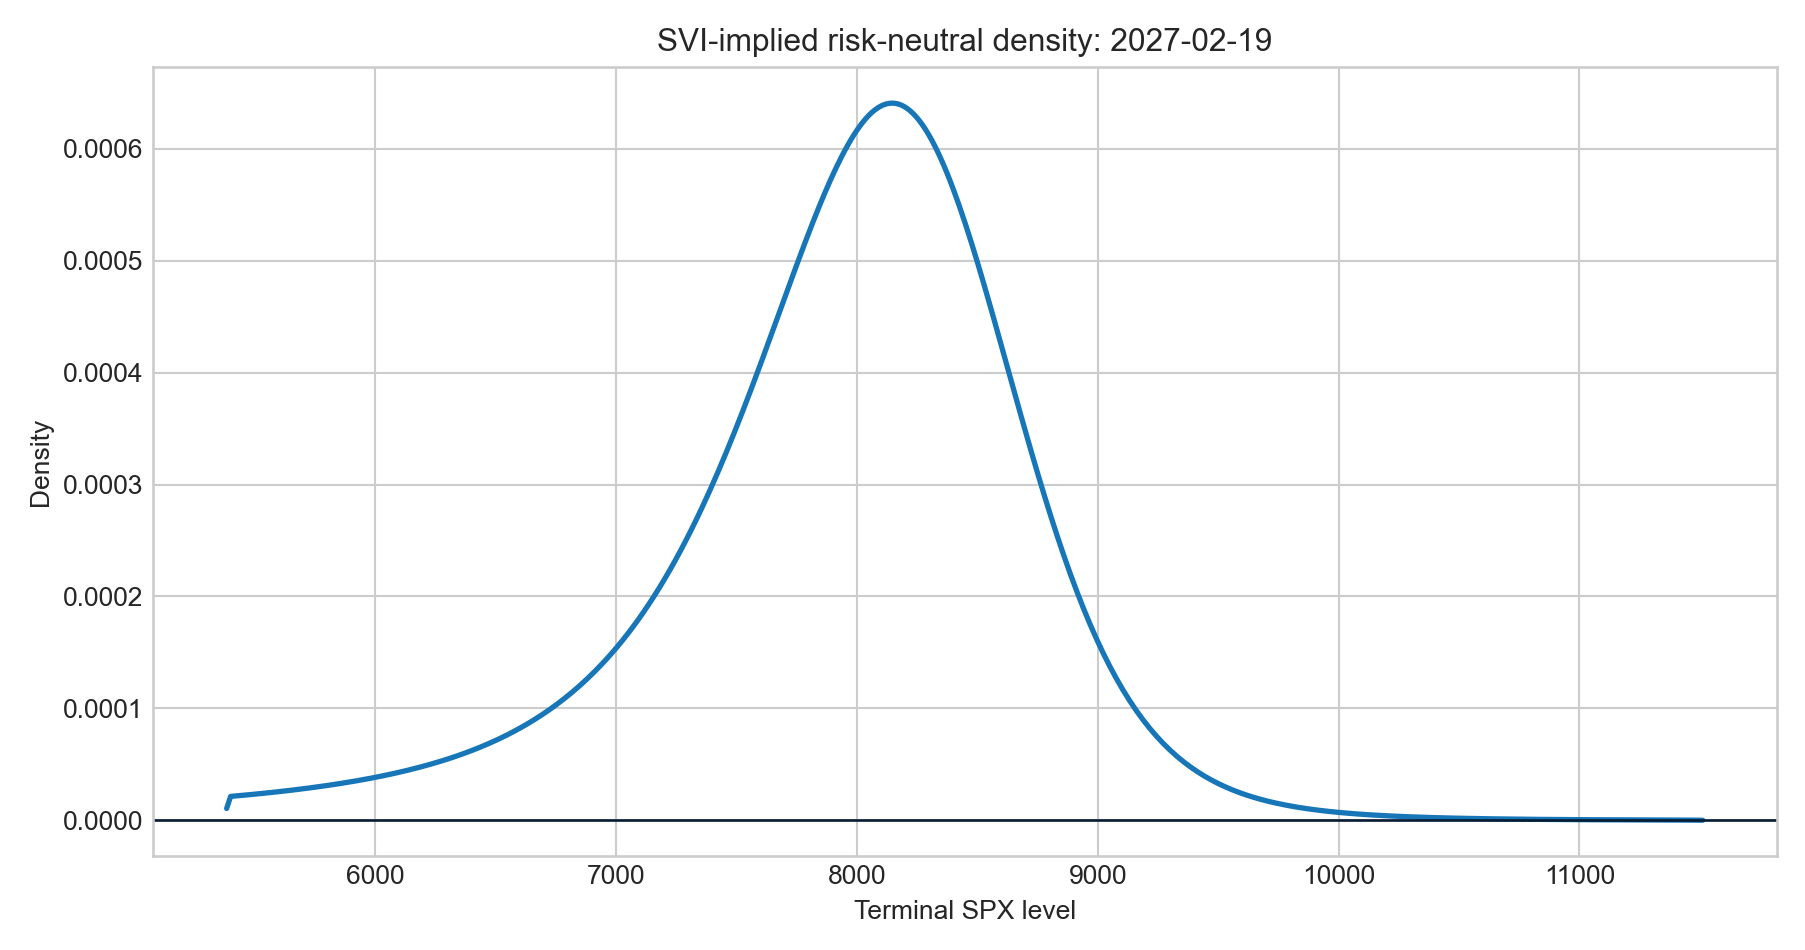
\includegraphics[width=.96\textwidth]{output/svi_state_price_density.png}
\caption{State-price-density diagnostic implied by equation \eqref{eq:g}.}
\end{figure}

\section{Heston structural compression}

Under the pricing measure, the Heston state follows
\begin{align}
 \dd S_t &= (r-q)S_t\dd t+\sqrt{v_t}S_t\dd W_t^S,\\
 \dd v_t &= \kappa(\theta-v_t)\dd t+\xi\sqrt{v_t}\dd W_t^v,
 \qquad \dd\langle W^S,W^v\rangle_t=\rho\dd t.
\end{align}
The parameters have distinct interpretations: $\kappa$ is mean-reversion speed,
$\theta$ long-run variance, $\xi$ volatility of variance, $\rho$ the return--variance
correlation, and $v_0$ initial variance. Calls are evaluated by Fourier inversion
of the characteristic function. Puts follow from parity.

Calibration minimizes price residuals normalized by Black vega,
\[
 \min_{\vartheta}\sum_{i\in\mathcal T}
 \left[
 \frac{P_i^{\mathrm{Heston}}(\vartheta)-P_i^{\mathrm{obs}}}
 {\max(\mathrm{Vega}_i,\epsilon)}
 \right]^2,
\]
so the objective is approximately an implied-volatility error rather than a
currency-weighted error dominated by expensive contracts. Five dispersed starting
points test local-solution sensitivity. Approximate standard errors use the local
least-squares Jacobian and should be read as curvature diagnostics, not as sampling
theory for dependent noisy quotes.

\begin{table}[ht]
\centering
\caption{Heston calibration and local curvature uncertainty.}
\resizebox{.82\textwidth}{!}{\begin{tabular}{lrrrrrr}
\toprule
parameter & estimate & local\_standard\_error & lower\_bound & upper\_bound & near\_boundary & selected\_start \\
\midrule
kappa & 2.84591 & 0.99035 & 0.05000 & 12.00000 & False & 5 \\
theta & 0.05587 & 0.00866 & 0.00500 & 0.60000 & False & 5 \\
vol\_of\_vol & 1.10912 & 0.10695 & 0.05000 & 3.00000 & False & 5 \\
rho & -0.67985 & 0.02961 & -0.99000 & 0.99000 & False & 5 \\
initial\_variance & 0.01682 & 0.00153 & 0.00500 & 0.60000 & False & 5 \\
\bottomrule
\end{tabular}
}
\end{table}

\begin{riskbox}[Feller condition]
The best fit has $2\kappa\theta-\xi^2<0$. The variance process remains definable, but
strict positivity is not guaranteed by the Feller sufficient condition. Imposing
that condition would change the empirical question and should be reported as a
separate restricted specification, not silently forced into the baseline.
\end{riskbox}

\section{Held-out comparison}

\begin{table}[ht]
\centering
\caption{Training and held-out errors. The holdout was excluded before calibration.}
\resizebox{\textwidth}{!}{\begin{tabular}{llrrrrr}
\toprule
model & sample & quotes & price\_rmse & iv\_equivalent\_rmse & iv\_equivalent\_mae & inside\_empirical\_noise\_fraction \\
\midrule
flat & holdout & 24 & 50.28291 & 0.04459 & 0.03827 & 0.08333 \\
heston & holdout & 24 & 5.44677 & 0.01464 & 0.00903 & 0.58333 \\
flat & train & 76 & 49.91876 & 0.04116 & 0.03606 & 0.18421 \\
heston & train & 76 & 4.32688 & 0.01421 & 0.00812 & 0.59211 \\
\bottomrule
\end{tabular}
}
\end{table}

On 24 held-out contracts, Heston reduces IV-equivalent RMSE from 0.04459 to 0.01464
and price RMSE from 50.28 to 5.45 index points. It places 58.3 percent of holdout
residuals inside the empirical noise band, versus 8.3 percent for the null. The
result rejects the claim that a maturity-level flat volatility is an adequate
cross-sectional description of this snapshot. It does \emph{not} establish that
Heston is the true data-generating process.

\begin{figure}[ht]
\centering
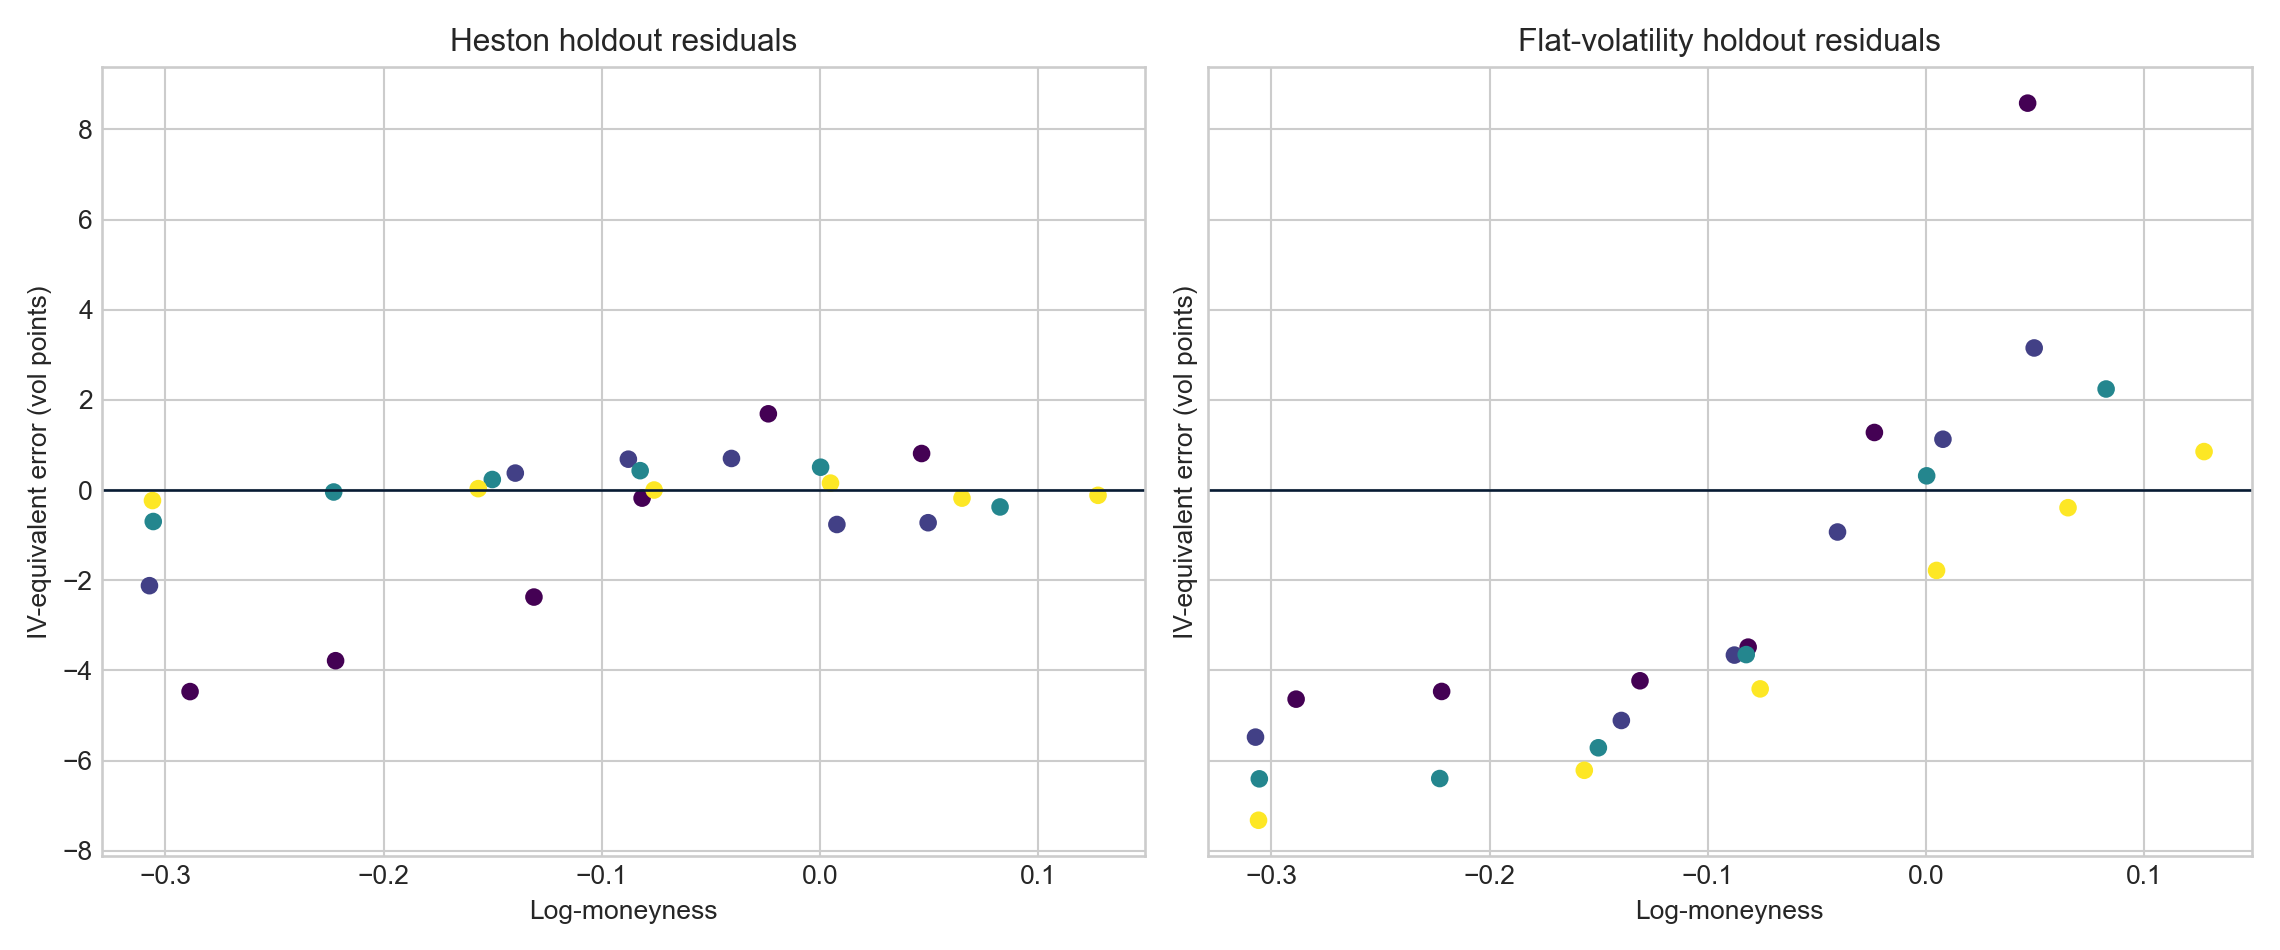
\includegraphics[width=.94\textwidth]{output/heston_holdout_residuals.png}
\caption{Held-out IV-equivalent residuals by log-forward moneyness.}
\end{figure}

\section{Model-risk register}

\begin{center}
\begin{tabularx}{\textwidth}{>{\bfseries}p{.20\textwidth}X X}
\toprule
Risk & Observable control & Remaining limitation\\
\midrule
Delayed transactions & Exact contract timestamps, common-session filter, immutable raw file &
Prices are asynchronous and not a synchronized NBBO.\\
Parity identification & Robust loss, liquidity weights, rate bounds, boundary flag &
Sparse call--put overlap can still bias forward and discount estimates.\\
Static arbitrage & Black bounds, dense SVI $g(k)$ test, Lee wings, calendar grid &
Finite-grid tests are numerical certificates on a declared domain, not global proofs.\\
Optimization & Multiple Heston starts and retained start-level table &
Agreement across starts does not eliminate common numerical or specification error.\\
Overfitting & Strike holdout and explicit flat-volatility null &
One date and deterministic split do not establish temporal stability.\\
Structural validity & Feller slack and local Jacobian uncertainty reported &
The best unrestricted fit violates the Feller sufficient condition.\\
\bottomrule
\end{tabularx}
\end{center}

\section{Reproduction and audit trail}

From the repository root, run
\begin{verbatim}
python projects/volatility_surface/run_research.py
python scripts/execute_notebooks.py notebooks/07_spx_surface_heston_validation.ipynb
powershell -ExecutionPolicy Bypass -File projects/volatility_surface/build_report.ps1
\end{verbatim}
The default research run uses the committed snapshot and is network independent.
Passing \texttt{--refresh} explicitly requests a new public-chain download. Each
generated file is covered by \texttt{output/manifest.sha256}; the provenance record
states whether the run used a refresh or the snapshot.

\section{Conclusion}

The strongest result is methodological, not ornamental. A defensible volatility
surface requires a chain of controls: contract convention, information timestamps,
parity identification, no-arbitrage price inversion, constrained smile geometry,
structural calibration, untouched observations, a meaningful null, and explicit
failure modes. In this snapshot the Heston compression is materially better than
flat volatility, while its negative Feller slack and the parity boundary identify
exactly where the structural story should not be oversold.

\begin{thebibliography}{9}
\bibitem{gatheraljacquier}
J. Gatheral and A. Jacquier,
\emph{Arbitrage-free SVI volatility surfaces}, Quantitative Finance 14(1), 2014.
\url{https://arxiv.org/abs/1204.0646}

\bibitem{heston}
S. L. Heston,
\emph{A Closed-Form Solution for Options with Stochastic Volatility with
Applications to Bond and Currency Options}, Review of Financial Studies 6(2), 1993.
\url{https://doi.org/10.1093/rfs/6.2.327}

\bibitem{oic}
Options Industry Council,
\emph{Understanding the Bid and Ask Prices for Options}.
\url{https://www.optionseducation.org/news/understanding-the-bid-and-ask-prices-for-options}
\end{thebibliography}

\end{document}
